\documentclass{article}
\usepackage{graphicx}
\usepackage{float}
\usepackage{booktabs}
\usepackage{amsmath}
\usepackage{amssymb}
\usepackage{iclr2026_conference,times}

\input{math_commands.tex}

\usepackage{hyperref}
\usepackage{url}

\title{The effect of batch size and momentum on the per-step performance of the Muon optimizer}

\author{
Do Duc Anh \\
\texttt{do.duc.anh@epfl.ch}
\AND
Julien Stalhandske \\
\texttt{julien.stalhandske@epfl.ch}
\AND
Missipsa M'Hamed Annane \\
\texttt{missipsa.annane@epfl.ch}
}

\iclrfinalcopy
\begin{document}
\maketitle

\begin{abstract}
Muon \citep{jordan2024muon} is a recently proposed optimizer that applies a Newton--Schulz orthogonalization to the momentum-buffered gradient of hidden weight matrices. We study, empirically, how the two hyperparameters that directly shape Muon's update -- the mini-batch size $B$ and the momentum coefficient $\mu$ -- affect its \emph{per-step} progress on a Wide ResNet 28--10 / CIFAR-10 benchmark. Sweeping a $6\times4$ grid ($B\in\{64,\dots,2048\}$, $\mu\in\{0.8,0.9,0.95,0.99\}$), we find that (i) Muon scales monotonically with $B$ in steps -- well past the bs=256 saturation point typical for vanilla SGD -- but (ii) at the cost of sample efficiency and $\sim$2\,pp of final test accuracy. The momentum coefficient is roughly insensitive at small $B$ but becomes the dominant hyperparameter at large $B$, where the EMA horizon must be matched to the (now short) training budget. We give a simple sample-horizon heuristic, $\tau \approx B/(1-\mu)$, that captures the observed best configurations.
\end{abstract}

\section{Introduction}
\label{sec:intro}

Most popular optimizers for deep learning -- SGD with momentum, Adam \citep{kingma2015adam}, AdamW \citep{loshchilov2019decoupled} -- update each parameter \emph{independently}. Muon \citep{jordan2024muon}, by contrast, replaces the gradient (or its momentum buffer) of every hidden weight matrix by its closest orthogonal matrix, computed efficiently by a quintic Newton--Schulz iteration. This makes Muon a practical, matrix-aware second-order-flavoured method, in the same family as Shampoo \citep{gupta2024shampoo} and modular-duality methods \citep{bernstein2024modular}, but with cost comparable to a few extra matmuls per step. Muon recently set speed records for training small GPT models and is increasingly used as a drop-in replacement for AdamW on hidden weights.

Two hyperparameters directly enter the update: the mini-batch size $B$ and the momentum coefficient $\mu$ of the EMA fed to the Newton--Schulz step. The optimization literature has a well-developed picture of $B$ for SGD/Adam: increasing $B$ reduces gradient variance and accelerates per-step progress, but only up to a critical batch size beyond which the scalability gain vanishes \citep{mccandlish2018empirical, shallue2019measuring}. Whether and how this picture transfers to Muon is a priori unclear: the orthogonalization step strips magnitude information from the update, which is precisely the dimension along which variance reduction operates. We therefore ask: \emph{at fixed compute, how does Muon's per-step progress depend on $B$, and how does $\mu$ interact with that scaling?}

\textbf{Contribution.} We run a controlled $6\times4$ sweep of $(B,\mu)$ for WRN-28--10 on CIFAR-10 (Section~\ref{sec:method}) and report (Section~\ref{sec:results}): (a) per-step convergence becomes monotonically faster with $B$ up to bs=2048, with no clear saturation in steps; (b) per-sample efficiency degrades sharply with $B$; (c) the optimal $\mu$ moves from a broad plateau around $0.9$--$0.95$ at small $B$ to a sharp $\mu^{\star}\!\approx\!0.95$ at large $B$, where both under- ($0.8$) and over-smoothing ($0.99$) hurt. We give a simple EMA-horizon argument for (c). Code at \texttt{plot.py}, \texttt{train.py}, \texttt{sweep.py}.

\section{Background and method}
\label{sec:method}

\paragraph{Dataset.} CIFAR-10 \citep{krizhevsky2009cifar}: 60{,}000 $32{\times}32$ colour images in 10 classes (50{,}000 train / 10{,}000 test). Pixels are normalised channel-wise; the training stream uses standard CIFAR augmentation ($4$-pixel reflection padding, random $32{\times}32$ crop, random horizontal flip), the test stream none.

\paragraph{Model.} Wide ResNet 28--10 \citep{zagoruyko2016wide,he2016deep}: a $3{\times}3$ stem conv, three stages of pre-activation residual blocks with widths $\{160, 320, 640\}$ and batch normalisation \citep{ioffe2015batch}, global average pooling, and a 10-way linear classifier ($\sim$36.5\,M parameters, no dropout, channels-last layout). WRN-28--10 is a standard CIFAR-10 backbone; our goal is not absolute accuracy but a fair, controlled comparison across $(B,\mu)$.

\paragraph{Muon.}
For each $2$D weight matrix $W$ with stochastic gradient $g_t$, Muon maintains an EMA-style buffer $m_{t} = \mu\, m_{t-1} + g_t$, forms a Nesterov-style direction $u_t = g_t + \mu\, m_t$, and updates
\begin{equation}
W_{t+1} \;=\; W_t \;-\; \eta\,s\, \mathrm{NS}_5(u_t),
\qquad
s = \max\!\big(1, (d_\mathrm{out}/d_\mathrm{in})^{1/2}\big),
\label{eq:muon}
\end{equation}
where $\mathrm{NS}_5$ is the $5$-step Newton--Schulz iteration of \citet{jordan2024muon} that maps a matrix $X = U \Sigma V^{\!\top}$ to a numerical approximation of $U V^{\!\top}$. Conv weights $(c_\mathrm{out}, c_\mathrm{in}, k_h, k_w)$ are reshaped to $(c_\mathrm{out}, c_\mathrm{in}k_hk_w)$ before $\mathrm{NS}_5$ is applied. Operationally, $\mathrm{NS}_5(u_t)$ is the closest-orthogonal matrix to $u_t$: Muon \emph{normalises every singular value to one}, so the update is purely a direction. Non-matrix parameters (biases, BN parameters, the stem conv and the final classifier) are trained with AdamW \citep{loshchilov2019decoupled}, as in the reference implementation.

\paragraph{Training pipeline and sweep.} We fix the Muon learning rate $\eta{=}0.02$, AdamW $\eta{=}3\!\times\!10^{-4}$ with $\beta{=}(0.9,0.95)$, weight decay $5\!\times\!10^{-4}$, and $5$ Newton--Schulz steps -- all defaults of the reference implementation. Every $(B,\mu)$ configuration trains for exactly $25$ \emph{epochs} (so all see the same data; smaller batches take more steps), with test accuracy logged twice per epoch. We sweep $B\in\{64,128,256,512,1024,2048\}$ and $\mu\in\{0.8,0.9,0.95,0.99\}$ -- a $24$-cell grid, single seed, $\sim$2.7\,h on an NVIDIA GTX 1660 Ti. $\mu{=}0.95$ is the reference value of \citet{jordan2024muon}.

\section{Results}
\label{sec:results}

\begin{figure}[!t]
\centering
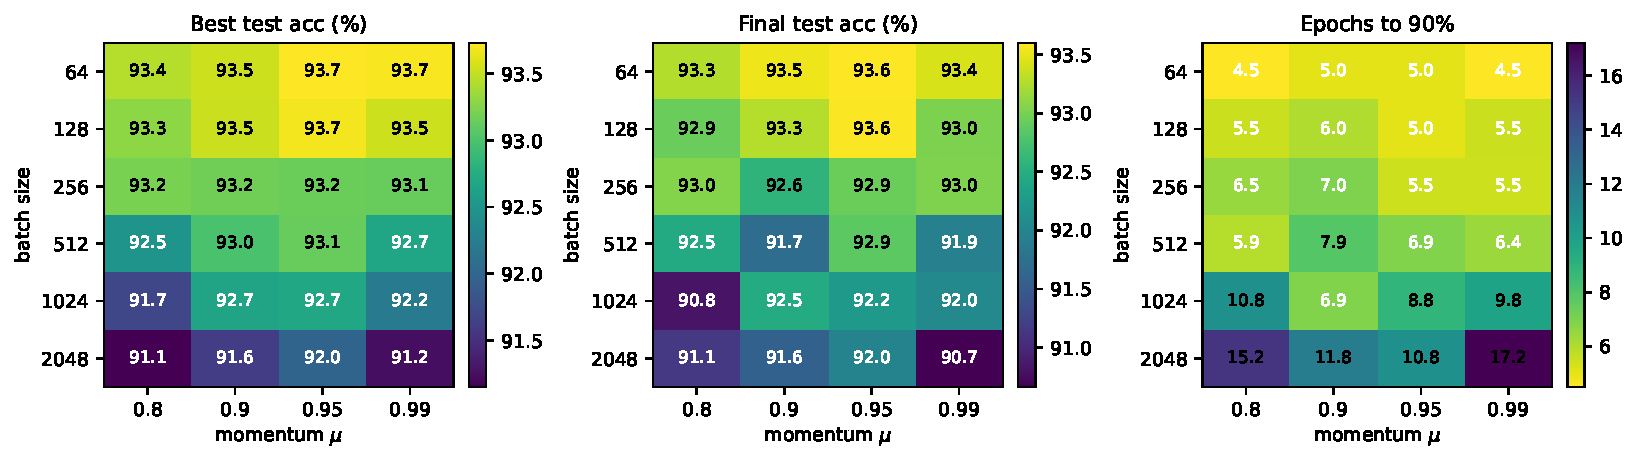
\includegraphics[width=\linewidth]{images/heatmap.pdf}
\caption{Sweep summary on the $(B,\mu)$ grid. \emph{Left:} best test accuracy during the 25-epoch run. \emph{Centre:} final-evaluation accuracy. \emph{Right:} epochs to first cross $90\%$ test accuracy. Best accuracy peaks at small/medium $B$; fastest configurations combine large $B$ with $\mu \in [0.9,0.95]$.}
\label{fig:heatmap}
\end{figure}

\begin{figure}[!t]
\centering
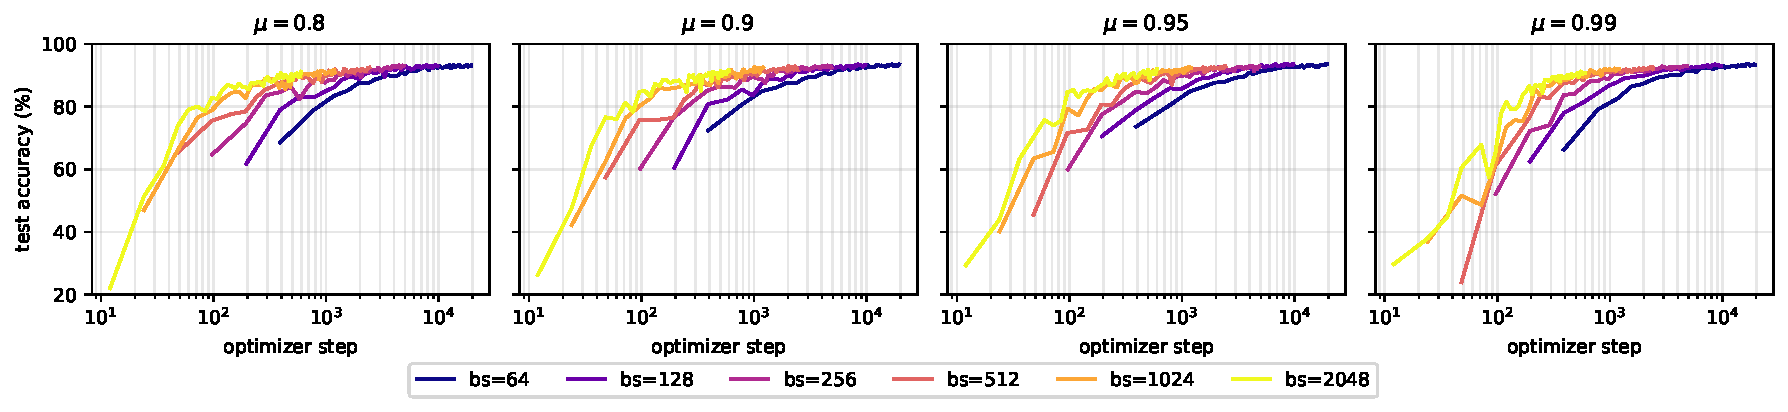
\includegraphics[width=\linewidth]{images/curves_per_step.pdf}\\[2pt]
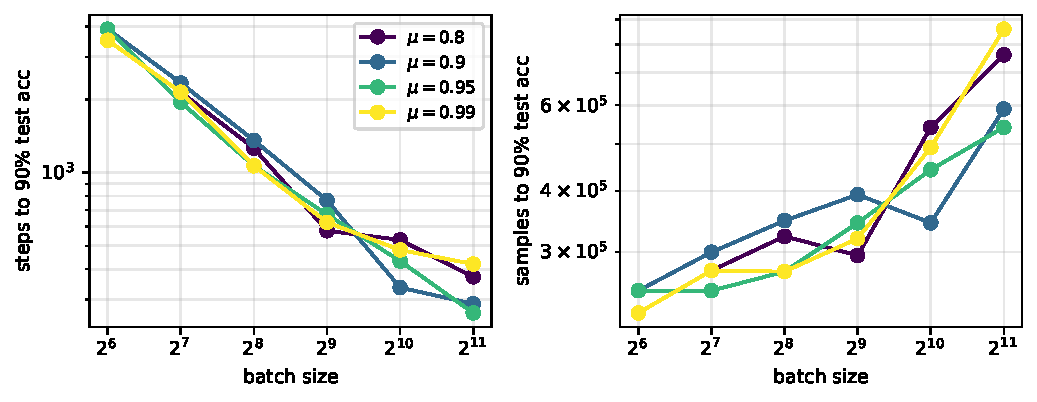
\includegraphics[width=0.85\linewidth]{images/sample_efficiency.pdf}
\caption{\emph{Top:} test accuracy vs.\ optimizer step (log), one panel per momentum; at fixed $\mu$ larger batches reach every accuracy threshold in fewer steps ($\sim$13$\times$ between bs=64 and bs=2048 at $90\%$). The $\mu{=}0.99$ panel shows the EMA-horizon pathology -- at bs=2048 the $\sim 1/(1-\mu){=}100$-step horizon eats $1/6$ of the budget. \emph{Bottom:} cost to first reach $90\%$ test accuracy in optimizer steps (left) and training samples (right), as a function of $B$, log--log. Steps-to-target falls sub-linearly with $B$; samples-to-target \emph{increases}.}
\label{fig:curves}
\end{figure}

\paragraph{Per-step performance scales monotonically with $B$.} At fixed $\mu$, larger batches reach every accuracy threshold in fewer optimizer steps (Fig.~\ref{fig:curves}, top). Steps to $90\%$ drop from $\sim$3{,}510 (bs=64) to $\sim$264 (bs=2048) at $\mu=0.95$ -- a $13.3\times$ reduction for a $32\times$ batch increase (Fig.~\ref{fig:curves}, bottom-left). A log--log fit gives $\mathrm{steps}_{90}\propto B^{-0.74}$: sub-linear, but \emph{no plateau within our range}. For SGD/Adam on similar CIFAR setups the critical batch size sits around $B^{\star}\sim 256$--$512$ \citep{shallue2019measuring}; Muon pushes that point at least an order of magnitude further. We attribute this to Muon's update being magnitude-free ($\mathrm{NS}_5(u_t)$ is orthogonal): SGD's main benefit from larger $B$ -- shrinking gradient \emph{magnitude} noise -- is moot for Muon, but the residual gain of cleaning up the singular \emph{directions} that $\mathrm{NS}_5$ picks out persists.

\paragraph{Sample efficiency degrades with $B$, and so does final accuracy.} Plotted in samples (Fig.~\ref{fig:curves}, bottom-right) the story flips: $90\%$ takes $\sim$250\,k samples at bs=128 but $\sim$540\,k at bs=2048 ($2.2\times$). Mean best test accuracy across the four momenta drops from $93.6\%$ (bs=64) to $91.5\%$ (bs=2048), a $2.1$\,pp loss (Fig.~\ref{fig:heatmap}, left). Two effects compound: large batches see fewer noisy iterates, weakening implicit regularisation \citep{goyal2017accurate}; and at fixed 25 epochs each large-batch update is asked to do strictly more work. Muon does not escape these well-known failure modes \citep{shallue2019measuring}.

\paragraph{The momentum coefficient becomes critical at large $B$.}
At bs=64 the four momenta land within $0.3$\,pp ($93.3$--$93.7\%$); at bs=2048 the spread is $0.9$\,pp ($91.1$--$92.0\%$), and the curvature in $\mu$ flips. At \emph{small} $B$ best accuracy is essentially flat in $\mu$: per-step variance is high, the orthogonalization recovers a clean direction every step, and the buffer adds little. At \emph{large} $B$ the optimum is sharply at $\mu{=}0.95$ and \emph{both} $0.8$ and $0.99$ are visibly worse. Under-smoothing ($\mu{=}0.8$, horizon $1/(1-\mu)\!\approx\!5$ steps) leaves $\mathrm{NS}_5$ acting on a still-noisy buffer; over-smoothing ($\mu{=}0.99$, $\sim$100-step horizon) outruns the budget ($600$ steps at bs=2048) so stale gradients dominate. A heuristic falls out: the buffer averages over $\tau \approx B/(1-\mu)$ \emph{samples}, and the configurations within $0.3$\,pp of the global best all sit in $\tau \in [10^3, 2\!\cdot\!10^4]$. This suggests retuning $1-\mu$ as $1/B$; $\mu{=}0.95$ sits in the middle of that band, which explains why it works across many workloads.

\section{Discussion and conclusion}

The two hyperparameters admit a unified picture. Muon's update is a normalised direction, so variance reduction from a larger $B$ keeps helping past the SGD plateau -- there is no magnitude-noise floor -- but at the usual large-batch price in samples and regularisation. The buffer has a sample-effective horizon $\tau \approx B/(1-\mu)$; keeping $\tau$ constant (not $\mu$) is the clean recipe for retuning momentum once $B$ is chosen, rather than treating $0.95$ as universal. Limitations: a single seed, fixed $\eta$, fixed-epoch budget, one model/dataset. A joint $(B,\mu,\eta)$ sweep on a transformer -- where Muon's appeal is sharpest -- is the most useful follow-up.

\section*{Statement of Contributions}
\textbf{We hereby state that all the work presented in this report is that of the authors.}

\bibliography{references}
\bibliographystyle{iclr2026_conference}

\end{document}
